\section{Elektrostatische Analyse}
Die \textbf{Elektrostatische Analyse} ist ein Hauptbestandteil des Designs von Hoch- und Mittelspannungsgeräten. Wird unter anderem für die Berechnung der Ersatzkapazität von elektrischen Komponenten und Leitungen verwendet.\\
\subsection{Grundgesetze}
\begin{tabular}[h]{ C{.23\linewidth} P{.53\linewidth} P{.22\linewidth} }
 {\vspace{0pt}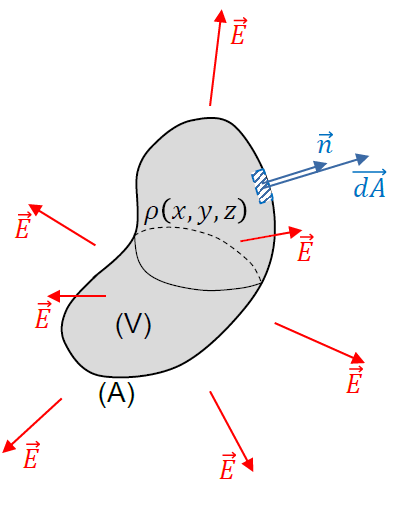
\includegraphics[width = 0.2\textwidth]{images/Gauss}} & \textbf{Gausssches Gesetz:} \newline \newline {\scriptsize Der Fluss des Vektors $\vec{D} = \varepsilon\cdot\vec{E}$ durch eine geschlossene orientierte Fläche (A) ist gleich der gesamten elektrischen Ladung Q, die von der Fläche (A) umgeben ist:}  \newline \[ \varoiint\limits_{(A)}\vec{D}\cdot\vec{dA} = Q \quad oder \quad \varoiint\limits_{(A)}\vec{E}\cdot\vec{dA} = \dfrac{Q}{\varepsilon} \] & {\vspace{2cm}{\footnotesize \textcolor{blue}{$\vec{D}$ - elektrische Flussdichte \newline $\vec{E}$ - elektrisches Feld \newline $\varepsilon$ - elektrische Permittivität}}} \\
{\vspace{0pt}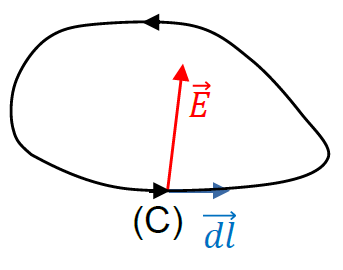
\includegraphics[width = 0.15\textwidth]{images/Wirbelfreiheit}} \newline \newline {\vspace{0pt}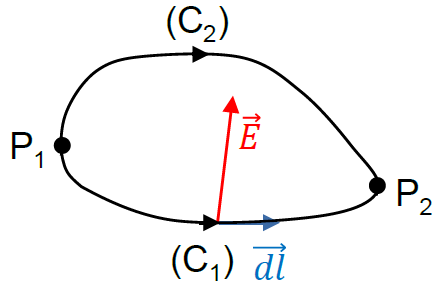
\includegraphics[width = 0.2\textwidth]{images/Wirbelfreiheit1}} & \textbf{Wirbelfreiheit des elektrostatischen Feldes:} \newline \newline {\scriptsize Das Kurvenintegral des elektrostatischen Feldes $\vec{E}$ über jede geschlossene orientierte Kurve (C) ist gleich null:} \newline \[ \oint\limits_{(C)}\vec{E}\cdot\vec{dl} = 0 \] \[
 \oint\limits_{(C)}\vec{E}\cdot\vec{dl} = \oint\limits_{\substack{P_1\\ (C_1)} }^{P_2}\vec{E}\cdot\vec{dl} - \oint\limits_{\substack{ P_1\\(C_2)} }^{P_2}\vec{E}\cdot\vec{dl} = 0\] & \\
 {\vspace{0pt}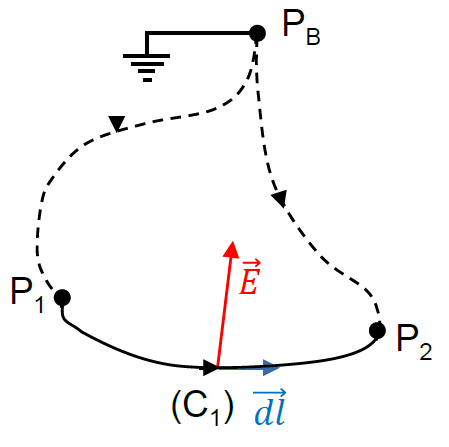
\includegraphics[width = 0.18\textwidth]{images/Skalarpotential}} & {\scriptsize Das elektrische Skalarpotential eines Punktes gegenüber dem Bezugspunkt ($P_B$):} \newline \newline \[ \varphi_{P_1} = \oint\limits_{P_1}^{P_N}\vec{E}\cdot\vec{dl}\quad und \quad \varphi_{P_2} = \oint\limits_{P_2}^{P_N}\vec{E}\cdot\vec{dl} \] \[ U_{P_1P_2} = \varphi_{P_1} - \varphi_{P_2} = \oint\limits_{P_1}^{P_2}\vec{E}\cdot\vec{dl} \] & \\
\end{tabular}
\begin{multicols}{2}
 \textbf{Poisson-Gleichung}  \[ \dfrac{\partial^2\varphi}{\partial x^2} +  \dfrac{\partial^2\varphi}{\partial y^2} + \dfrac{\partial^2\varphi}{\partial z^2} = -\dfrac{\rho}{\varepsilon} \]
 \textbf{Laplace-Gleichung}  \[ \dfrac{\partial^2\varphi}{\partial x^2} +  \dfrac{\partial^2\varphi}{\partial y^2} + \dfrac{\partial^2\varphi}{\partial z^2} = 0 \]
 \\
 \\
 \textbf{Randbedingungen} \\
 \textcolor{blue}{Der geerdete Rand:} \[\varphi = 0\] 
 \textcolor{blue}{Der Rand mit bekannten Potential:} \[ \varphi = A, \]
 \textcolor{blue}{Der Rand der Symmetrie:} \[ \dfrac{\partial\varphi}{\partial n} = 0\] 
 %TODO: Divergenz und Gradient noch ergänzen
\end{multicols}
\clearpage
